%%%%%%%%%%%%%%%%%%%%%%%%%%
% Technische Umsetzung   %
%%%%%%%%%%%%%%%%%%%%%%%%%%
\section{Technische Umsetzung}

\begin{frame}{Intelligentes Messsystem - iMSys I}
   \begin{center}
      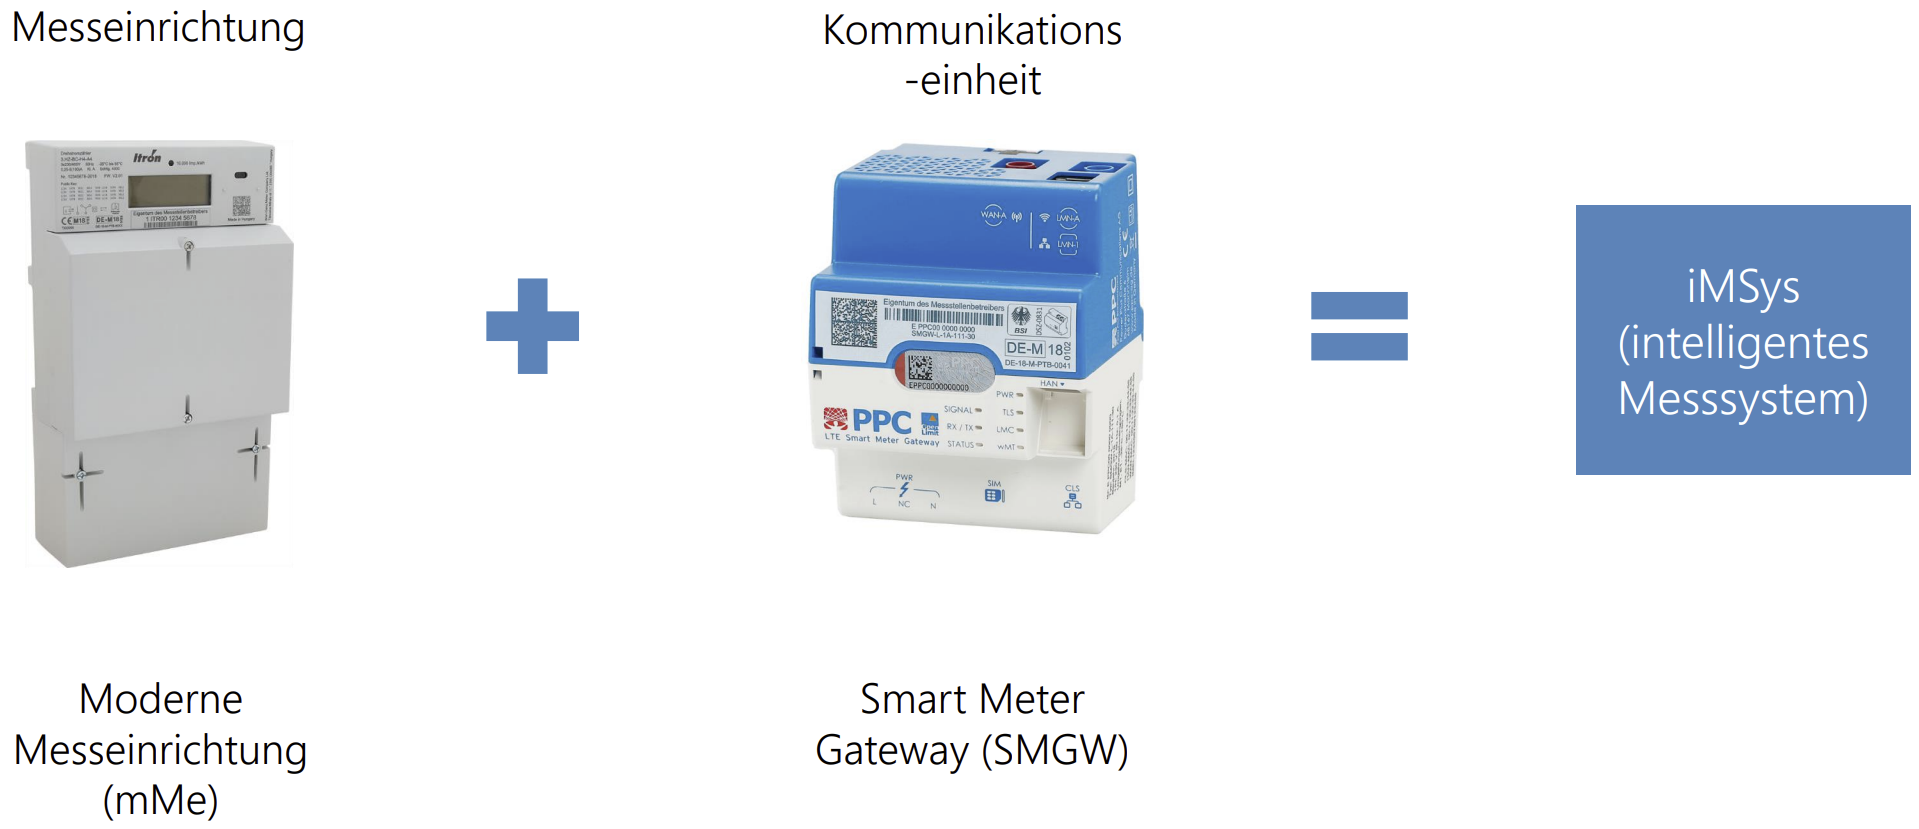
\includegraphics[width=10cm]{images/iMSys.png}
   \end{center}
   Quelle: FfE e.V.\cite{FFE2020imsys}
\end{frame}

\begin{frame}{Intelligentes Messsystem - iMSys II}
   \begin{center}
      \begin{minipage}{0.34\textwidth}
         \centering
         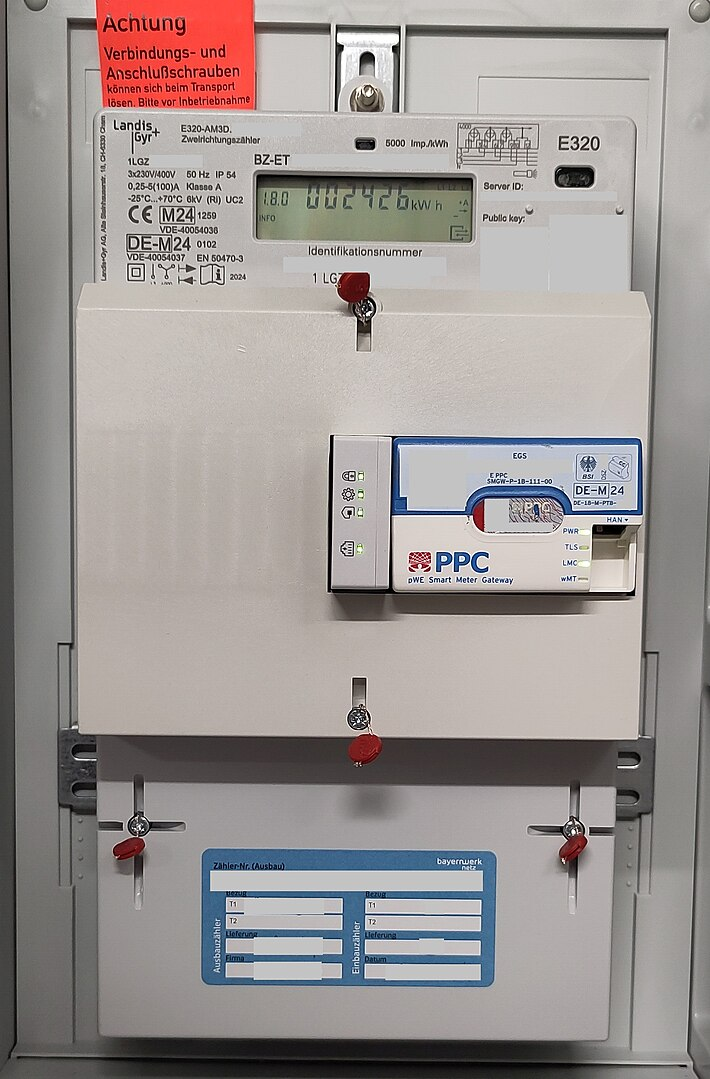
\includegraphics[width=\linewidth]{images/SmartMeter.jpg}
      \end{minipage}
      \begin{minipage}{0.64\textwidth}
         \centering
         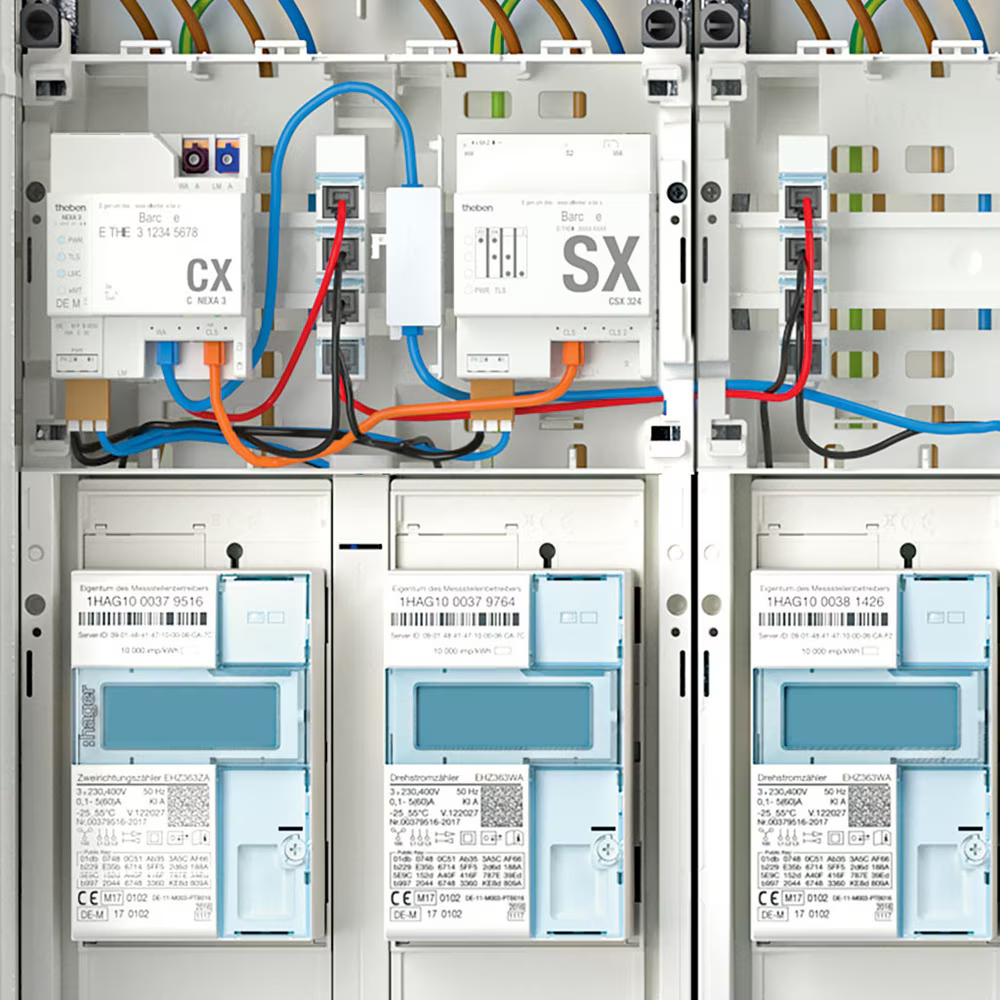
\includegraphics[width=0.8\linewidth]{images/technikzentrale.png}
      \end{minipage}
   \end{center}
   Quellen: \href{https://commons.wikimedia.org/wiki/File:2024-SmartMeter.jpg}{Wikipedia}, Hager
\end{frame}

\begin{frame}{Smart Meter Gateway}
   \begin{center}
      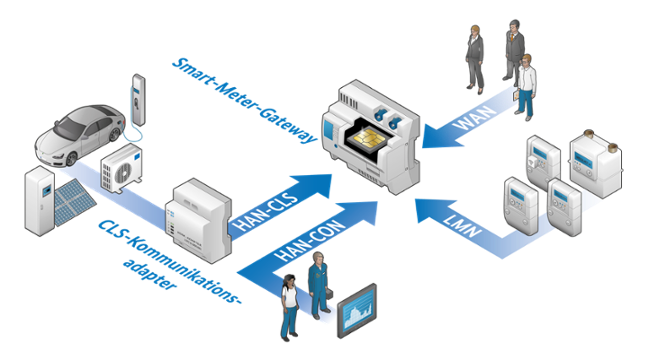
\includegraphics[width=10cm]{images/smartmetergateway.png}
   \end{center}
   Quelle: BSI\cite{FFE2020imsys}
   ,Detailinfos zu HAN VDE FNN\cite{VDEFNNimpulsDigitaleSchnittstellen2023}
\end{frame}

\begin{frame}{Zertifizierte Komponenten}
   \begin{itemize}
      \item TR-03109-1 \href{https://www.bsi.bund.de/DE/Themen/Unternehmen-und-Organisationen/Standards-und-Zertifizierung/Smart-metering/Smart-Meter-Gateway/Zertifikate24Msbg/produkte.html}{Smart-Meter-Gateways - SmGW} (13)
      \item TR-03109-5 \href{https://www.bsi.bund.de/DE/Themen/Unternehmen-und-Organisationen/Standards-und-Zertifizierung/Smart-metering/Kommunikationsadapter/Zertifikate/Zertifikate_TR_03109-5_node.html}{Steuerboxen - CLS} (8)
   \end{itemize}
   \vspace{0.3cm}
   \begin{center}
      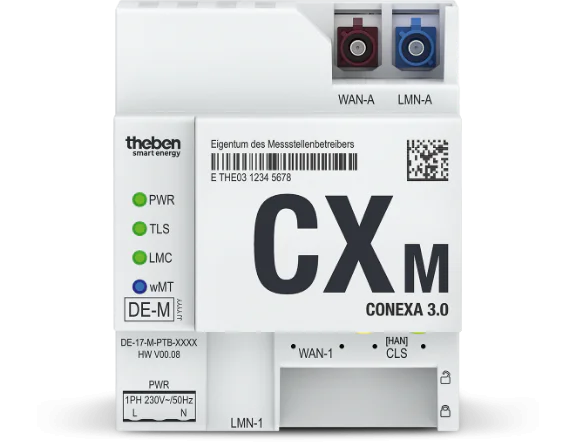
\includegraphics[height=4cm]{images/Theben_CXm.png}
      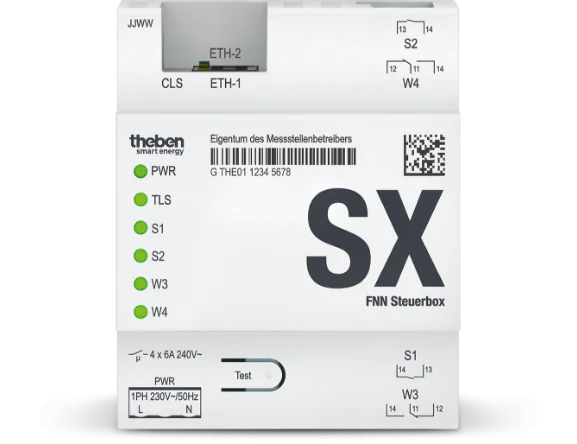
\includegraphics[height=4cm]{images/Theben_SX.png}
   \end{center}
\end{frame}

\begin{frame}{Netzdienliche Steuerung}
   \begin{block}{\enquote{Dimmen} von Verbrauchern $>4,2\,\text{kW}$}
      \begin{itemize}         
         \item Begrenzung der elektrischen Leistung auf 4,2 kW...
         \item ...Wärmepumpen z.B. Heizstab deaktivieren (SG-Ready)
         \item ...Wallbox teilt Maximalleistung 4,2 kW mit (PWM-Signal)
         \item ...Speicher Netzbezug auf 4,2 kW drosseln
      \end{itemize}
   \end{block}
   \begin{block}{Verbraucher mittels Preissignalen steuern}
      \begin{itemize}
         \item Fixe Zeitfenster mit drei Netzentgeltstufen
         \item Laden des E-Autos in Schwachlastzeiten
         \item Bevorzugt laden des Speichers in Schwachlastzeiten
         \item Entladen des Speichers in Hochlastzeiten
         \item Heizungspuffer \enquote{füllen} + Warmwasserbereitung
      \end{itemize}
   \end{block}
   \vspace{0.3cm}
\end{frame}

\begin{frame}
   \frametitle{Roll-Out Quoten Q4/2024}
   \centering
   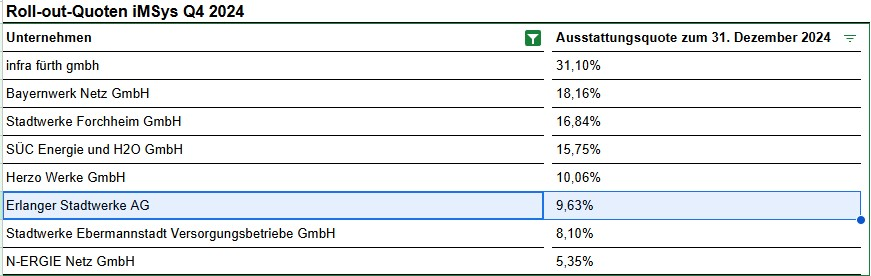
\includegraphics[width=0.95\paperwidth]{images/Roll-Out-Quoten.jpg}
   Quelle: Bundesnetzagentur\cite{BNetzA2025RolloutQuoten}
\end{frame}
